\section{Marco te\'orico}

\subsection{Machine learning}
\begin{frame}
\frametitle{Aprendizaje m\'aquina(Machine learning)}

\begin{figure}[h]
\centering
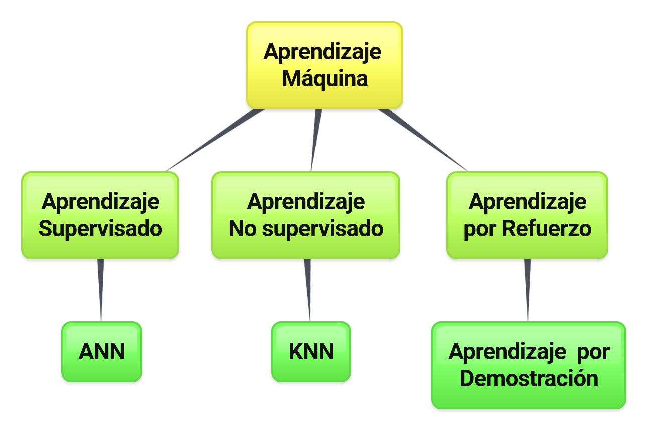
\includegraphics[width=0.8\columnwidth]{Imagenes/Aprendizaje.eps}
\caption{Clasificación del aprendizaje m\'aquina
 \cite{9780471056690, 9780387310732}.}
\label{fig:ClasifML}
\end{figure}

\end{frame} 


\subsection{Grafos}
\begin{frame}
\frametitle{Grafo dirigido}

\begin{figure}[h]
\centering
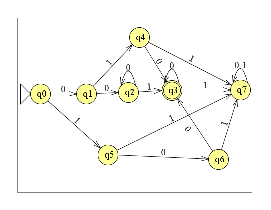
\includegraphics[width=0.7\columnwidth]{Imagenes/GrafoDirigido.eps}
\caption{Ejemplo de un grafo dirigido.}
\label{fig:grafod}
\end{figure}

\end{frame} 


\subsection{Tipos de datos}
\begin{frame}
\frametitle{Tipos de datos}

\begin{figure}[h]
\centering
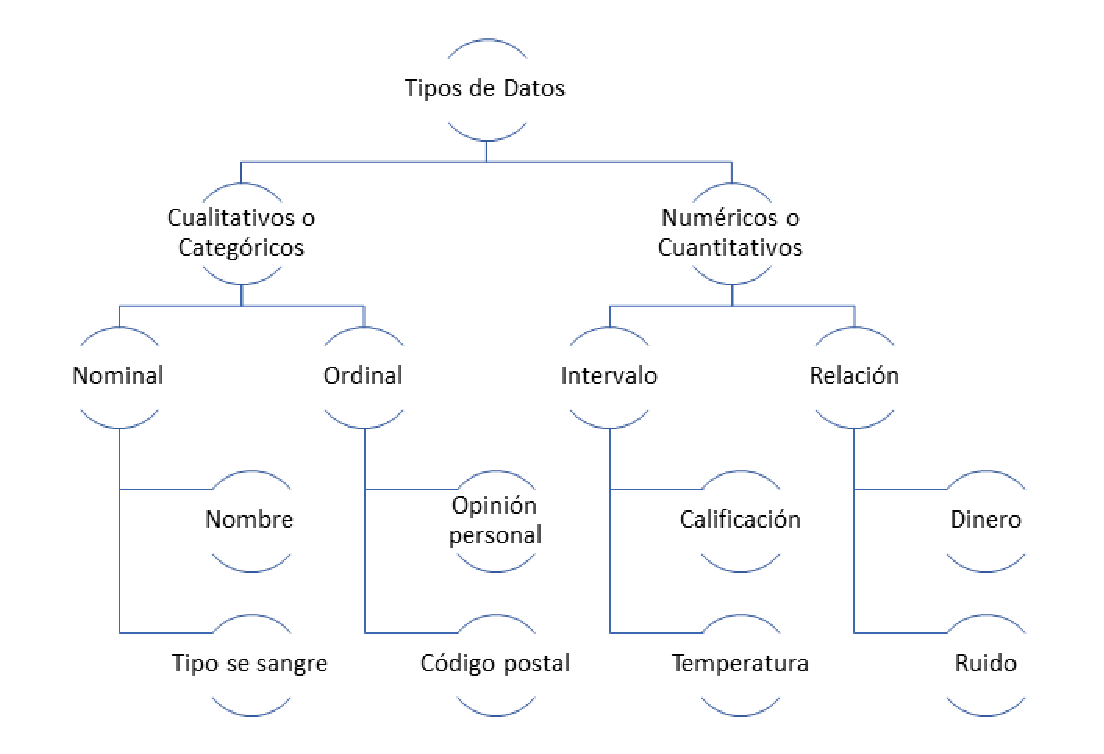
\includegraphics[width=0.85\columnwidth]{Imagenes/clasifnums.eps}
\caption{Clasificaci\'on de tipos de datos.}
\label{fig:clasnums}
\end{figure}

\end{frame}